%!TEX program = xelatex
\documentclass{article}
 % ---------------------------------------------------------------------
\usepackage{xeCJK}
\usepackage{fontspec}
\setCJKmainfont[BoldFont={黑体}]{宋体}
% ---------------------------------------------------------------------
\usepackage{geometry}
\geometry{a4paper, top=25mm, left=30mm, right=25mm, bottom=30mm,
         headsep=10mm, footskip=12mm}
% ---------------------------------------------------------------------
\usepackage{graphicx}
\usepackage{amsmath}
\usepackage{amsfonts}
\usepackage{url}
\usepackage{listings}
% Listings Style
\lstset{
	numberstyle=\footnotesize, 
	basicstyle=\footnotesize\ttfamily,
	numbers=left, 
	numbersep=5pt, 
	frame=single
}
% ---------------------------------------------------------------------
\title{计算机视觉:人脸识别}
\author{赵阳旻,14307130067\\复旦大学计算机科学与技术学院\\https://github.com/yangminz/tensorface}
\date{2016 12}
 % ---------------------------------------------------------------------
\begin{document}

\maketitle
\tableofcontents

\bigskip
这份课程的实验代码请见:https://github.com/yangminz/tensorface 所需的环境与相关说明可以参考README.md文件。

\section{历史的行程}

人脸识别对于人类而言并不困难。在我们的计算机视觉课上,陈老师曾经拿过几个名人的照片给我们识别,陈晓旭、布什……知道他们的人都可以认出照片对应的人,即使不认识照片对应的人,也能看出两张照片是不是描述的同一个人。科学研究发现,甚至只出生了一天到三天的婴儿,也能够识别不同的人脸,即便婴儿谁都不认识。人脸识别的机制与人类大脑的梭状回面孔区有密切关系,我们有时候会在电视节目的奇闻异事中看到患有“脸盲症”的人,他们大脑的相应区域都出现了一些障碍,所以人脸识别能力比较低。但是对于计算机而言,人脸识别并不是一件简单的事,尤其是在人脑的人脸识别机制尚未探清的情况下,我们主要依赖统计方法来帮助计算机进行人脸识别。\\

在历史上,第一个真正意义上的人脸识别是在1965年完成的,Woody Bledsoe, Helen Chan Wolf, Charles Bisson都成为了人脸识别的先驱。他们运用几何方法,人工标注面部特征,计算出两眼之间的距离比例、眼与鼻的角度等几何特征,在他们的数据集上获得了不错的效果。但是几何方法由于其局限性太大,并没有走到21世纪。\\

到了1991年,基于主成分分析的特征脸方法被MIT的Matthew A. Turk和 Alex P. Pentland提出了。这对于人脸识别而言是一个里程碑式的进步,这样基于统计的方法要优于基于几何结构的方法,一时间成为了人脸识别的主流,一直持续到现在,依然作为人脸识别中非常重要的方法。\\

在21世纪,随着人工神经网络摆脱过去的阴霾,开始走向深度学习,基于卷积神经网络的一系列计算机视觉领域的突破给人脸识别带来了新的方法。Krizhevsky在ImageNet上用卷积网络大杀四方,前后时间内人脸识别也运用了卷积网络的技术。到现在,深度学习已经成为计算机视觉领域内的一股有力的支流,像Face++这样的公司展露头角。

\section{卷积神经网络}

\subsection{人工神经网络}

人工神经网络的数学基础是Kolmogorov和Arnold在50年代发展起来的函数逼近定理:\\

\noindent
\fbox{\begin{minipage}{\linewidth}
$\Phi (y)$是单调有界连续增函数,其中$y = f(x_1, x_2, \ldots, x_n)$只是一个有界闭子集上的连续函数,则:\\
$\forall \epsilon > 0$,存在正整数$H$和$c_j, \theta_j$,有$w_{ij},i,j \in \{ 1,2,\ldots,n\}$,
\[ g(x_1,x_2,\ldots,x_n) = \sum_{j=1}^H c_j \Phi \left( \sum_{i=1}^n w_{ij} \cdot x_i - \theta_j \right) \]
\[ s.t. \max |f(x_1,x_2,\ldots,x_n) - g(x_1,x_2,\ldots,x_n)| < \epsilon\]
其中$\Phi(\cdot)$在实际运用中一般为$\tanh, sigmoid$这些常见的非线性函数。
\end{minipage}}

\bigskip

在Kolmogorov定理的基础上,复杂函数逼近的方法得到了提高。于是到60年代时,在梯度下降算法的帮助下,感知机模型被提出。到了80年代,人工神经网络被建立起来,而1986年Hinton提出的Back Propagation算法更是通过求导的链式法则解决了高层网络难以反馈求导的问题。到了21世纪,硬件的发展使得人工神经网络的运算速度大为提升。

\subsection{历史与发展}

在21世纪,20世纪末发展的神经网络模型的变种——卷积神经网络开始随着机器性能的提升而展现威力。1998年,Yann LeCun在他的惊世传奇\emph{Gradient-based learning applied to document recognition}中提出了第一个真正意义上的卷积神经网络模型——LeNet-5,Yann LeCun利用这个模型在Mnist手写数据集识别上取得了突破性的进展,而这个数据集至今仍作为机器学习入门的数据集在使用。\\

在2006年,Hinton则提出了他的惊世骇俗之神作\emph{Reducing the dimensionality of data with neural networks},点明了深层网络对于特征学习能力的优越性,这为后来如火如荼的深度学习奠定了基础。\\

到了2012年,Hinton的亲传弟子Krizhevsky提出了他的CNN模型AlexNet,在ImageNet上一鸣惊人,以极大的差距击败第二名摘得桂冠。同时,他的论文\emph{Imagenet classification with deep convolutional neural networks}也将永远被人们铭记,因为这标志着人工智能的研究开始进入深度学习阶段。\\

但是,我们也可以看到,实际上真正的理论创新在20世纪就已经止步不前了,如今深度学习能够如此繁花似锦、烈火烹油,完全得益于硬件的加速。回顾历史,我们可以发现,人工智能这一领域,基本上始终是围绕着神经网络为中心展开的,虽然其中有SVM异军突起,但终究扭转不了历史的行程。

\subsection{卷积神经网络的原理}

数学上的离散卷积公式是这样的:\\

\noindent
\fbox{\begin{minipage}{\linewidth}
若$\xi$与$\eta$是独立的随机变量,且都取非负整数值,概率分布分别是${a_k}$和$b_k$,则随机变量$\zeta = \xi + \eta$的概率分布为:
\[ P\{\zeta = r\} = \sum_{k = 0}^r P\{ \xi=k, \eta=r-k \} = \sum_{k = 0}^r a_k b_{r - k} \]
\end{minipage}}

\bigskip

而实际上神经网络的原理和卷积公式的关联并不密切。以1维的卷积网络为例:\\

\begin{center}
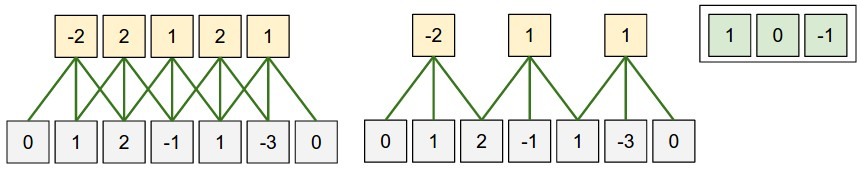
\includegraphics[width=0.8\linewidth]{fig09.jpg}
\end{center}

可以看到它实际上只是一个窗口上的加权平均。但是这样的网络,却在图像处理方面有着巨大的优势。\\

众所周知,神经网络对于复杂特征的学习具有非常的优势,但是在人脸识别这样复杂的工程中,如果使用传统的神经网络会带来一个非常严重的后果——模型参数过多。由于图片作为输入时,每个像素上的值都是一个输入,而图片上的像素点又是何其多,给每个输入分配一个权重,这样的训练未免太强机器所难。因此,解决这个问题的方法是减小网络参数,在每层网络上使用全局参数,这就是LeCunn的论文的想法。\\

\begin{center}
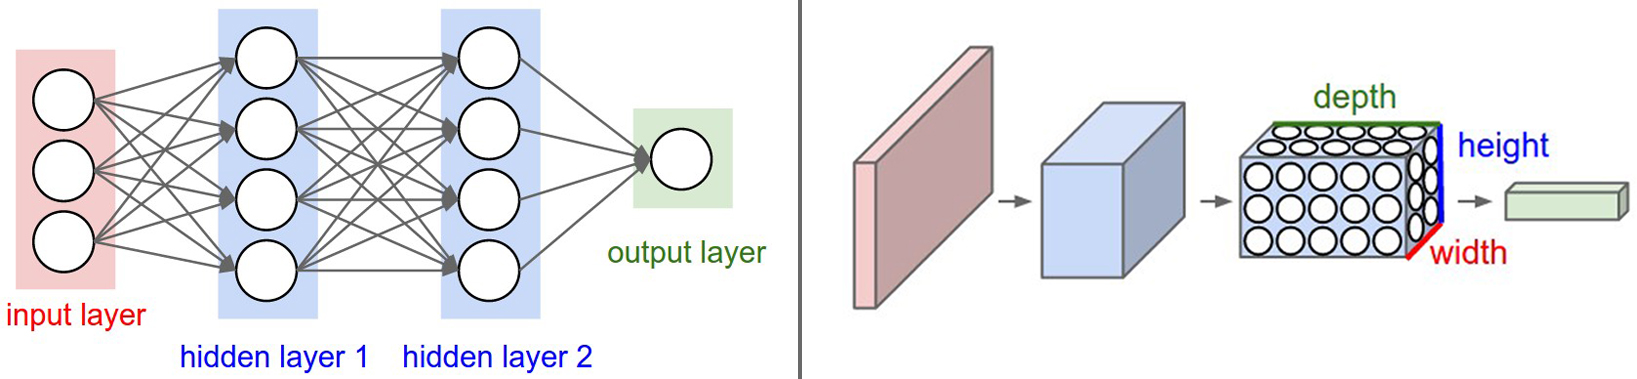
\includegraphics[width=0.8\linewidth]{fig10.jpg}
\end{center}

上面这张图出自Stanford University的课程cs231n。这张图描述了传统的神经网络与卷积网络的差异。左图是一张3层的全连接网络,可以看到即便输入只在$\mathbb{R}^3$,但到输出层的时候保存的参数已经不少了,如果输入达到$1920 \times 1080$这样的级别,那么参数更是爆炸性的多,训练根本无从下手。\\

但是卷积网络则可以避免这个弊端。可以看到左图的这个网络,对于一个RGB三色通道的$\mathbb{R}^{3 \times H \times W}$的图像输入,卷积网络通过卷积滤波器(卷积核)提取同一张图像的不同变换下的特征,需要保存的权重矩阵的数量之后滤波器深度那么多,这样大大减小了模型的参数量。

\subsection{卷积操作}

卷积网络的关键之一自然是\textbf{卷积操作}。我们依然借用cs231n的图来做如下说明:

\begin{center}
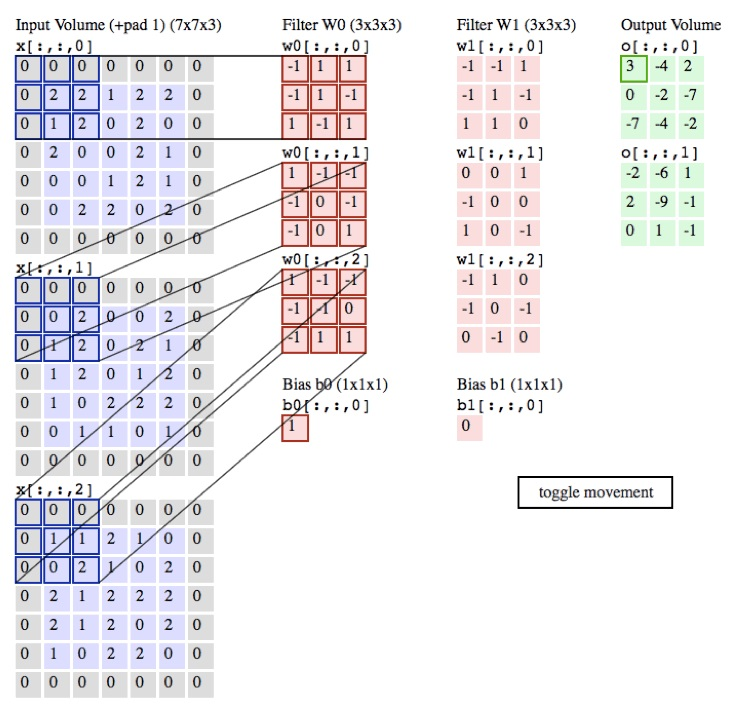
\includegraphics[width=0.8\linewidth]{fig11.jpg}
\end{center}

上图是一个RGB三色通道$\mathbb{R}^{3 \times H \times W}$的图像输入。左边三张蓝色矩阵是图像的三色通道,中间有两列粉红色的$\mathbb{R}^{3 \times 3 \times 3}$的卷积滤波器矩阵$\mathbf{W_0}, \mathbf{W_1}$,分别对应着右边两张绿色的输出矩阵。在这里要注意,卷积滤波器的深度必须要和图像输入的深度一致,这是显而易见的,在上图中为3。卷积滤波器的个数可以任意设定,这里是2。\\

进行卷积操作时,$\mathbf{W_0}$3个深度的矩阵分别遍历3个深度上的图像输入,并且做加权平均,然后将三个数值加到一起,作为卷积层的一个数值。在上图中,对应关系已经标注得很清晰了。\\

\subsection{卷积操作的实验}

可见通过这样的模型,确实能够有效地减少模型的参数。我们可以通过传统网络背后的Kolmogorov定理来理解卷积网络,可以认为这是一种特殊的参数设定。但是问题来了,虽然我们知道卷积网络能够减少网络参数,而且也是Kolmogorov定理的一种变形,但是它为什么能够工作,这一问题回答得还不足够清楚。\\

一种通俗而且形象的解释是类比于人脑中的神经元。人脑中的神经元的结构实际上更类似于卷积网络而非传统的全连接网络:

\begin{center}
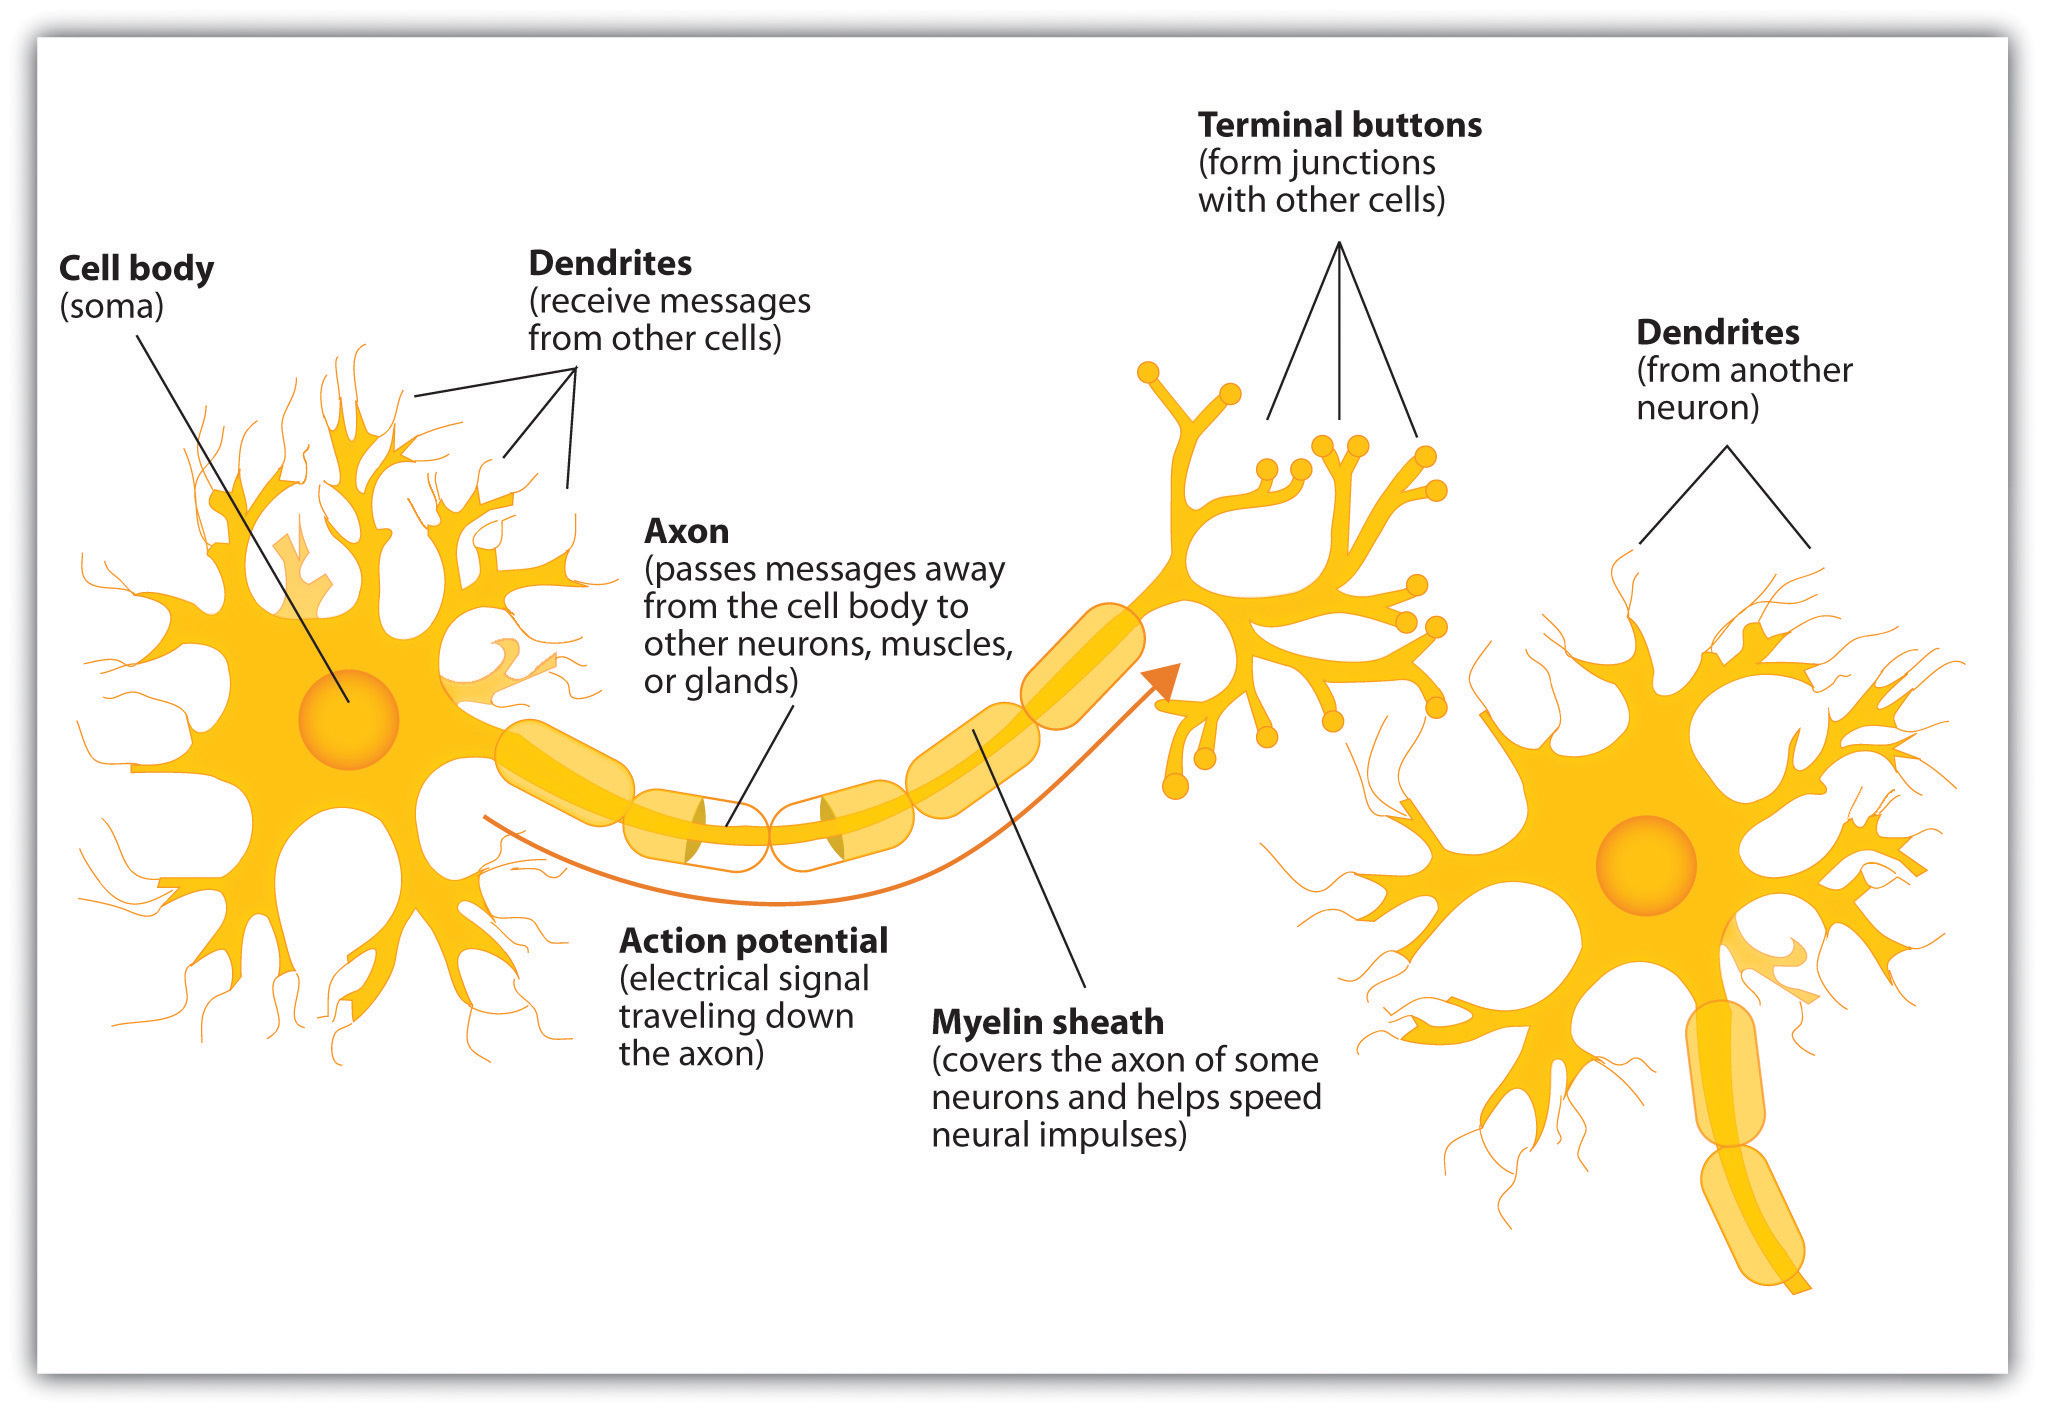
\includegraphics[width=0.8\linewidth]{fig12.jpg}
\end{center}

人脑的神经元也是局部连接的,并不是一个神经元与所有其他神经元相连,因此卷积网络和人脑更相似,所以特征学习能力更强。实际上这也是可以理解的,表现在图像上就是卷积网络更能抓住局部特征,无视图像远方的干扰信息,因此能有更强的特征学习能力。\\

我在实验中利用Keras写了这样一个简单的卷积网络\\

 \begin{lstlisting}[caption={Keras CNN}, language=python]
model = Sequential()

# Building: conv1 - tanh - maxpooling
model.add(Convolution2D(filter1, conv_side, conv_side,
    border_mode='same', 
    subsample = (2, 2), dim_ordering='tf', 
    input_shape=(h, w, 1)))
# print model.output_shape
model.add(Activation('tanh'))
model.add(MaxPooling2D(pool_size=(pool_side, pool_side)))

# Building: conv2 - tanh - maxpooling
model.add(Convolution2D(filter2, conv_side, conv_side))  
model.add(Activation('tanh'))  
model.add(MaxPooling2D(pool_size=(pool_side, pool_side)))  
# model.add(Dropout(0.25))  

# Building: flat - dense - tanh - dense - softmax
model.add(Flatten())  
model.add(Dense(1000)) #Full connection  
model.add(Activation('tanh'))  
# model.add(Dropout(0.5))  
model.add(Dense(SUBJECT_NUM))  
model.add(Activation('softmax')) 

sgd = SGD(lr=sgd_lr, decay=sgd_decay, momentum=sgd_momentum, nesterov=True)
model.compile(loss='categorical_crossentropy', optimizer=sgd)
return model
\end{lstlisting}

训练好以后保存了模型以及参数。然后将图像输入这个训练好的模型中,将第一次卷积的中间结果取出,经过归一化到$[0, 255]$等处理,还原出图像:\\

\begin{center}
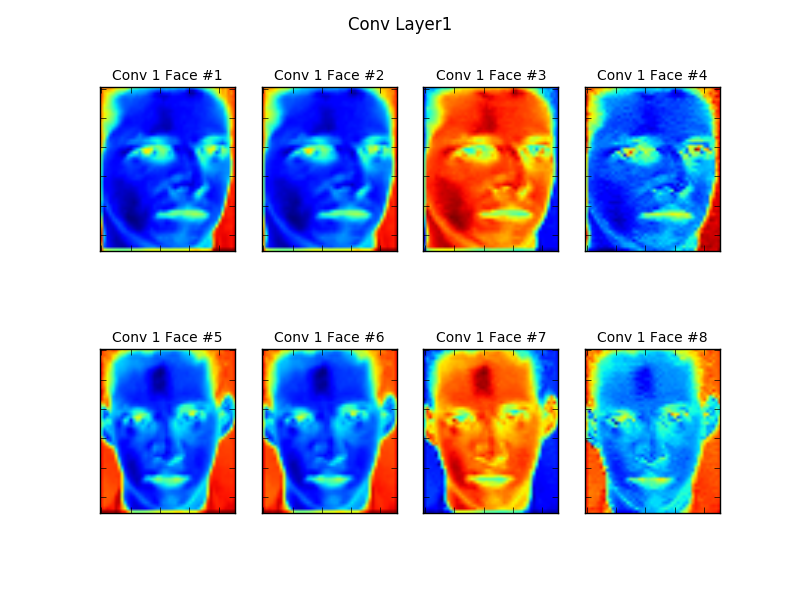
\includegraphics[width=0.8\linewidth]{../image/conv1.png}
\end{center}

上下两行4张图分别是某个人的脸经过卷积滤波器,在卷积层的前4深度上的图像。可以看到,不同深度的滤波器实际上在抓取不同的特征,比如卷积滤波器$\mathbf{W_0}$抓到的特征$(0, 0)$这张脸在图像上表现为蓝色,而$\mathbf{W_2}$抓到的特征$(0, 2)$则表现为红色。

\subsection{池化及实验}

除了卷积操作以外,总是成对出现的操作有池化(pooling):

\begin{center}
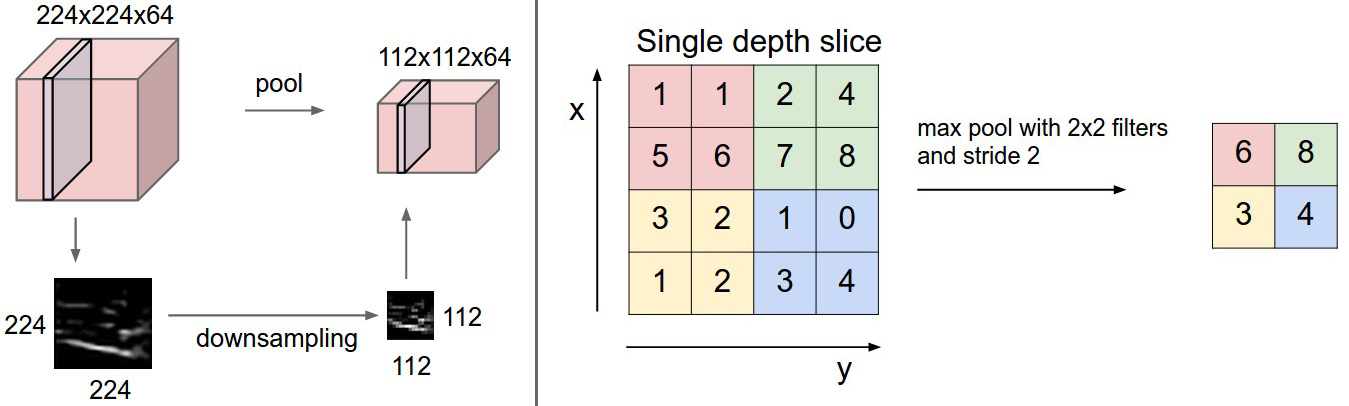
\includegraphics[width=0.8\linewidth]{./fig14.jpg}
\end{center}

我理解池化是进一步丢弃数据的过程。上图是一个最大池化的例子,在每个池化窗口中,选出最大值作为池化层的数据。这样的丢弃数据实际上是具有某种“随意性”的,这给反向求导带来了不可捉摸的困难,但是现在大家写卷积网络基本都用机器学习的框架,所以也就无所谓了,把精力集中在前向传播上。总之,这种“随意性”以及无法精确的反向求导,能够比较好地对抗过拟合问题。\\

\begin{center}
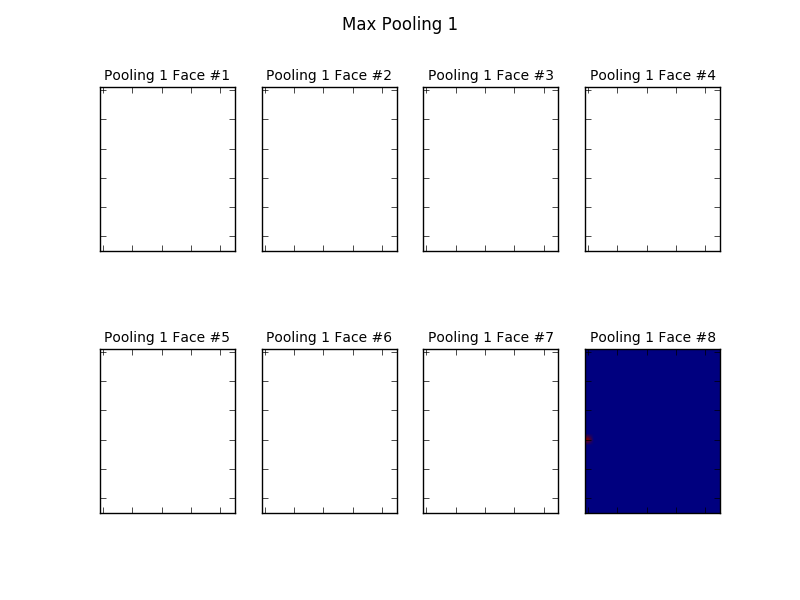
\includegraphics[width=0.8\linewidth]{../image/pool1.png}\\
\end{center}

可以看到第一层池化层的结果如上图所示,这个结果其实我自己也没怎么搞明白为什么会丢掉这么多的数据,但是到第二层卷积与池化之后就变得正常了。\\

\begin{center}
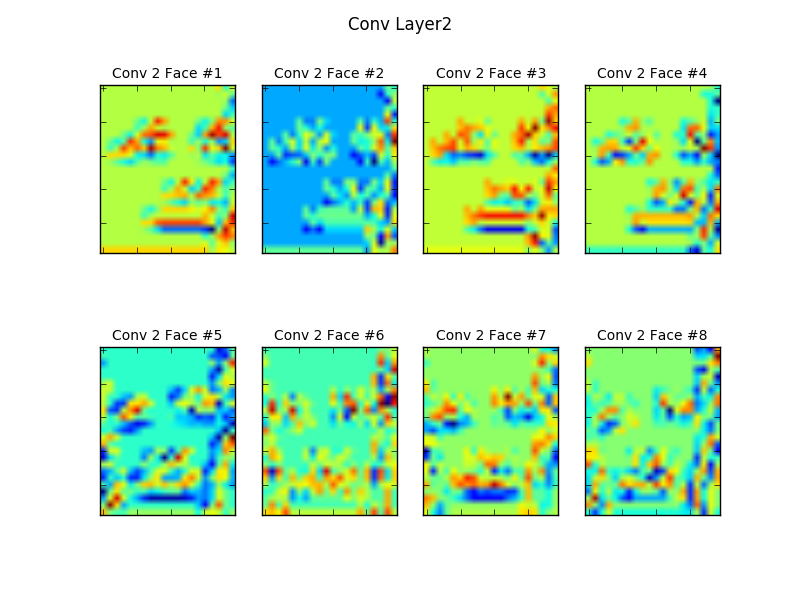
\includegraphics[width=0.8\linewidth]{../image/conv2.png}
\end{center}

这是第二层卷积。可以看到,经过一次卷积与池化以后,到第二层卷积层时,卷积层输入已经被大大削减,而且基本保留了原图像的重要特征:眼、耳、鼻。可知,卷积网络的学习能力是很强的。\\

\begin{center}
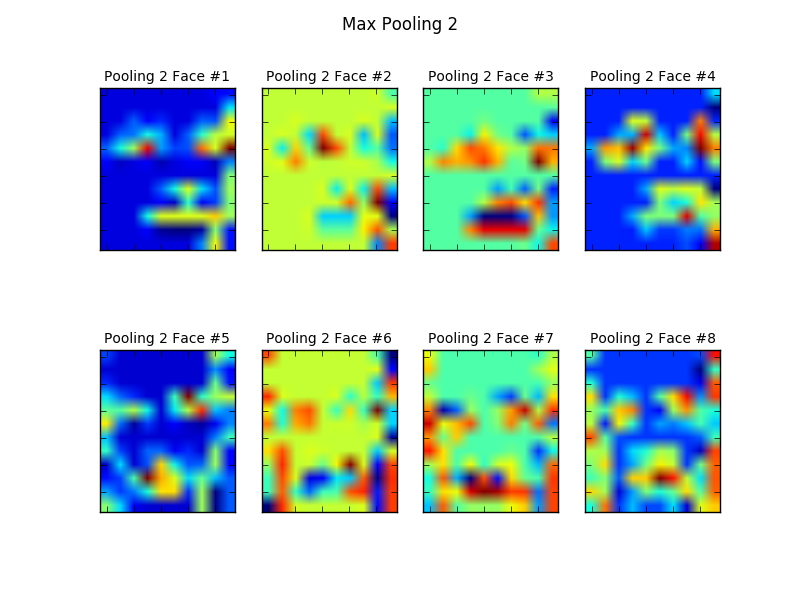
\includegraphics[width=0.8\linewidth]{../image/pool2.png}\\
\end{center}

可以看到,到第二层池化以后,特征更加明显,并且输入更小。也就是说,采用卷积与池化,实际上是一个在尽可能保留特征的前提下,不断减小图像规模的过程。从结果来看,训练好的卷积网络将这两点结合得很好,到第二次池化时,也就是上面这张图,图像的抽象层次基本上只保留了眼、耳、鼻这样的特征了。到这一步,接下来再用一个传统网络作为分类器,代价就并不高了。所以我在模型中经过两层卷积以后就进行了全连接分类。\\

其实我觉得可以从类比\textbf{积分中值定理}的角度来理解卷积和池化。\\

\noindent
\fbox{\begin{minipage}{\linewidth}
设$f$和$g$都在区域$\Omega$上可积,且$f$在$\Omega$上连续,$g$在$\Omega$上不变号,则:\\
\[ \exists \xi \in \Omega, s.t. \]
\[ \int_{\Omega} f \cdot g dV = f(\xi) \int_{\Omega} g dV\]
\end{minipage}}

\bigskip

可以看到,积分中值定理实际上是在函数连续的条件下选取了一个代表$f(\xi)$来代表整个区域$\Omega$。而对于一张合理的图像而言,也应该具有某种\textbf{连续性}。所以,对于每一个局部区域,卷积实际上是找了一个\textbf{代表}来进行降维。卷积操作也可以这样粗糙地理解,它是用不同的代表(特征)来表征一个局部区域。\\

需要注意的是,到这里我们可以看到,不论是卷积操作亦或是池化操作,都基于输入在局部区域上保持着“连续性”。这个特点应该是一张合乎情理的图像所与生俱来的,也是卷积网络之所以能在计算机视觉领域大展神威的原因之一。但是,如果我们做一个简单的思想实验,对于图像进行外延:如果我们的技术能够超越离散进化到连续的程度,那么就能找到这样一种图像,它“处处不连续、处处不可微”,也就是类似于\emph{Dirichlet}函数,并且在取值上更加混沌的图像,那么卷积网络应该是无能为力的。

\subsection{影响网络的超参数}

影响卷积网络的超参数有很多,隐藏层的大小、卷积层的个数、卷积窗口的大小、步长、是否做padding(0或1)……在一篇合格的文献中基本上都能够找到相关超参数的性质分析,而且我也没做改变超参数的实验,所以就没必要一一说明了。\\

在这里我只想简单说一下网络层数的影响。因为卷积与池化都是局部操作,所以每一层只获得了前一层的局部信息,但是显然层数累加的时候这样的局部信息也在累加。也就是说,层数越高,每一层获取的图片信息“密度”就越高,它越能从“局部感知”走向“全局感知”。

% ---------------------------------------------------------------------

\section{主成分分析}

相比于与人工智能始终紧密联系的神经网络,主成分更像是传统的数理统计方法。因此它并不像神经网络那样充满了不可知的“玄学”(甚至于有人将其比喻为“黑箱”),主成分分析从构想,到数学推导,再到结果,都一气呵成,一俟现世就已经成熟,充满了优雅。如果打一个不恰当的比喻,主成分像是Alexis de Tocqueville笔下的旧贵族,浴沂风雩咏而归,而神经网络则像是他笔下的民主人,终日乾乾,夕惕若厉。

\subsection{主成分分析的历史}

主成分分析(PCA)由Karl Pearson在1901年首创,距今已经有超过100年的历史了,当时大清还没亡。它是为了解决统计力学问题应运而生的,后来被广泛地运用在信号处理等领域。到现在,PCA在复杂统计数据的处理上享有赫赫威名,人脸识别就是其应用之一,这部分的历史在第一节就已经讲过了。

\subsection{PCA的本质}

PCA在本质上是一个特征分析多元统计分布的方法,它要寻找高维的数据空间上对方差影响最大的方向。从几何上讲,样本点$\mathbf{x_1}, \ldots, \mathbf{x_n}$在$\mathbb{R}^d$上形成了椭圆状的云团,PCA要找到就是这个云团的主轴,也就是散布最大的方向,从而实现对空间的降维。\\

在前一节卷积网络中,我们有提到过,实际上CNN也实现了降维,不过它并不直白,而且保留了图像的特征。在PCA中,降维是直观的,目的是找到正确的方向,投影样本数据以后依然能够有效地分类。

\subsection{数学推导}

假定我们有人脸数据集$\mathbf{X} = \{\mathbf{x_1}, \mathbf{x_2}, \cdots, \mathbf{x_n} \} \in \mathbb{R}^{n \times d}$

\subsubsection{降到$\mathbb{R}^0$的场合}

$\mathbb{R}^0$场合是指,我们希望找到一个$\mathbf{x_0} \in \mathbb{R}^{d}$点就能代表所有的人脸样本点。理论上讲是所有的人脸样本点都投影到这个点,但从实际效果上讲就是找到$\mathbf{x_0}$能最好地代表人脸样本就行。或者说:与所有样本之间的距离的平方和越小越好:
\[ J_0(\mathbf{x_0}) = \sum_{k = 0}^n || \mathbf{x_0} - \mathbf{x_k} ||^2 \]

拆开目标函数:
\[ J_0(\mathbf{x_0}) = \sum_{k = 1}^n || (\mathbf{x_0} - \mu ) - ( \mathbf{x_k} - \mu ) ||^2 \]

\[  = n\cdot || \mathbf{x_0} - \mathbf{\mu} ||^2 + \sum_{k = 0}^n || \mathbf{x_k} - \mathbf{\mu} ||^2  - 2 \cdot ||\mathbf{x_0} - \mathbf{\mu} || \cdot  \sum_{k = 0}^n ( \mathbf{x_k} - \mathbf{\mu} ) \]
\[  = n \cdot || \mathbf{x_0} - \mathbf{\mu} ||^2 + \sum_{k = 0}^n || \mathbf{x_k} - \mathbf{\mu} ||^2  \]
右边一项并不依赖于$\mathbf{x_0}$是常量,所以左边一项取均值$\mu$时目标函数取极小值。\\

由此可以知道,在$\mathbb{R}^0$场合下,最能代表所有人脸样本的就是均值点。但是$\mathbb{R}^0$显然是降维过头了,到这个程度已经没有方向可言了,分开数据更无从谈起,所以下面要考虑到投影到$\mathbb{R}^1$的场合。

\subsubsection{$\mathbb{R}^1$的场合}

现在考虑降到一维的情况,也就是将样本点投影到一条经过均值点的直线上,让这根直线上的投影点来代表全体数据点:
\[ \mathbf{x} = \mathbf{\mu} + a \cdot \mathbf{e} \]
在这里,标量$a$反应了投影点对均值的偏离程度,$\mathbf{e}$是单位方向向量。\\

现在,我们希望最小化投影点和实际点之间的差异:\\
\[ ||(\mathbf{\mu} + a_k \cdot \mathbf{e}) - \mathbf{x_k}|| \]
所以构造平方误差函数:\\
\[ J_1(a_1, \cdots, a_n, \mathbf{e}) = \sum_{k=1}^n ||(\mathbf{\mu} + a_k \cdot \mathbf{e}) - \mathbf{x_k}||^2  \]

展开处理:\\
\[ J_1 = \sum_{k=1}^n a_k^2 - 2\sum_{k=1}^n a_k \mathbf{e^T}(\mathbf{x_k - \mu}) + \sum_{k=1}^n ||\mathbf{x_k - \mu}||^2 \]

这样就可以对$a_k$求偏导:\\
\[ \frac{\partial J_1}{\partial a_k} = 2a_k - 2\mathbf{e^T}(\mathbf{x_k - \mu}) = 0 \Rightarrow a_k = \mathbf{e^T}(\mathbf{x_k - \mu}) \]

从几何上讲,这告诉我们向量$\mathbf{x_k}$只要向直线$\mathbf{e}$做垂直投影,就能得到最小方差。接下来的问题是:如何找到直线$\mathbf{e}$的最优方向?这就需要引入散布矩阵的概念:\\
\[ \mathbf{S} = \sum_{k=1}^n (\mathbf{x_k - \mu})(\mathbf{x_k - \mu})^T \]

散布矩阵实际上是协方差矩阵的$n-1$倍。用散布矩阵来描述目标函数:\\
\[ J_1(\mathbf{e}) = -\mathbf{e^TSe} + \sum_{k=1}^n ||\mathbf{x_k - \mu}||^2 \]

用Lagrange乘子法求$||\mathbf{e}||=1$的条件极值:\\
\[ u = -\mathbf{e^TSe} + \lambda \left( \mathbf{e^Te} - 1 \right) \]

对$\mathbf{e}$求偏导:\\
\[ \frac{\partial u}{\partial \mathbf{e}} = 2\mathbf{Se} - 2\lambda\mathbf{e} = 0 \]
\[ \Rightarrow  \mathbf{Se} = \lambda\mathbf{e} \]

所以方向向量一定和特征向量平行!要让$\mathbf{e^TSe} = \lambda\mathbf{e^Te} = \lambda$最大,就要选取散布矩阵最大的特征值所对应的特征向量作为方向向量。

\subsubsection{高维场合}
如果要提取到高维空间$d'$(更多)的特征向量呢?
\[ \mathbf{x = \mu} + \sum_{i=1}^{d'} a_i \mathbf{e_i} \]
取散布矩阵前$d'$个最大的特征值所对应的特征向量就行了。\\

此外,由于散布矩阵实对称,所以这些特征向量相互正交。

\subsection{numpy实验}

为了更直观地展现PCA的效果,我用numpy写PCA时,也像CNN一样提取了两个中间结果:

\begin{center}
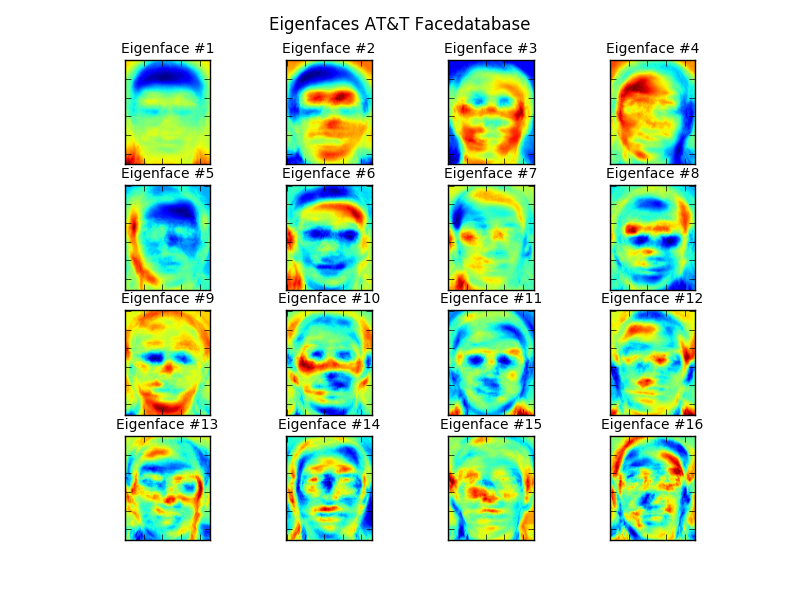
\includegraphics[width=0.8\linewidth]{../image/eigenfaces.png}\\
\end{center}

这张图是将选出来的特征向量都还原为图片所得的结果,可以看到每一个特征向量都抓取到了不同的对象的面部特征,这些特征和CNN一样主要集中在眼、耳、鼻等五官上。

\begin{center}
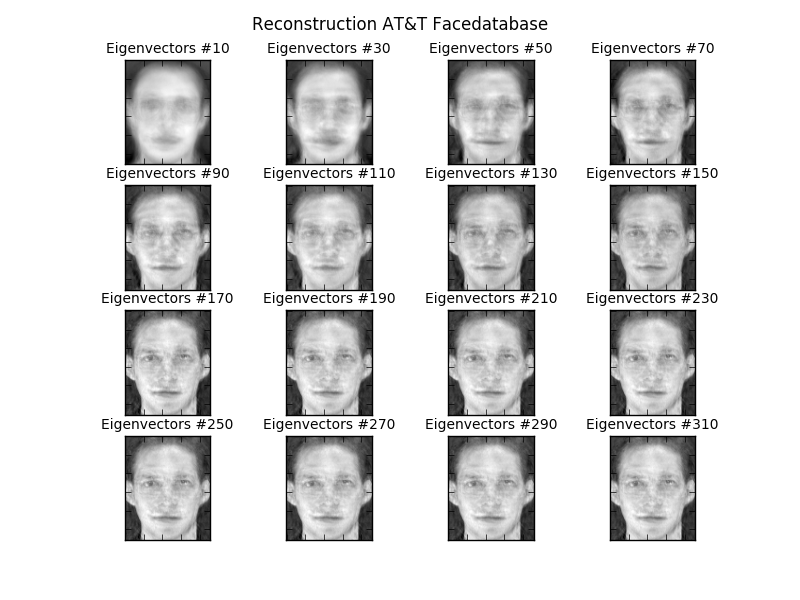
\includegraphics[width=0.8\linewidth]{../image/eigenvectors.png}\\
\end{center}

这张图则对比不同特征向量的数量的影响。在实验中选择了不同数量的特征向量,也就是投影的正交坐标的个数,然后将它们还原成人脸。可以看到,特征向量越多,人脸就越清晰。这是当然的,投影越多越接近原图,当取全部特征向量做投影时,实际上也就恢复成原来的人脸了。实际上这方面和矩阵的秩有关,因为特征值的个数与矩阵的秩相同,深究下去的话,可能会发现灰度图像与它的矩阵的秩之间有深刻的联系。

% ---------------------------------------------------------------------

\section{人脸识别:既成熟又不成熟的技术}

上面两个模型,在AT\&T与Cambridge大学联合做出来的AT\&T数据集\footnote{http://www.cl.cam.ac.uk/research/dtg/attarchive/facedatabase.html}上都有近乎$100\%$的识别率,难道我们就可以说人脸识别到现在是一项成熟的技术了吗?非也,实际上在更复杂的课题中,模型的表现并不总是令人满意。

\subsection{更复杂的应用场景}

就单拿静态照片的识别而言,主要有两个重大的问题:光照变化和姿态变化。\\

不同光照条件下的照片会给图像带来巨大的灰度相对分布,这样引起的光照变化带来的同一张人脸之间的差异甚至可能超过其他的人脸之间的差异,也就是类内差异大于类间差异。下图是经过剪裁的Yale的人脸数据集\footnote{http://vision.ucsd.edu/~iskwak/ExtYaleDatabase/ExtYaleB.html},可以看到光照变化的影响:

\begin{center}
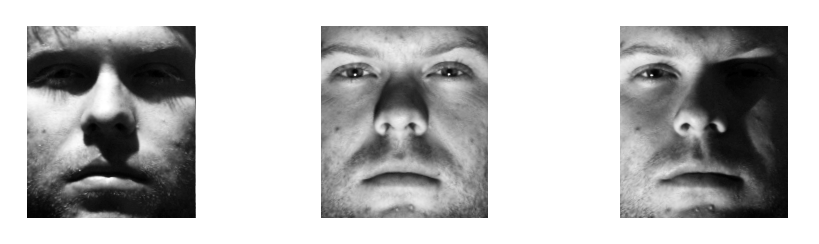
\includegraphics[width=0.35\linewidth]{./fig25.png}\\
\end{center}

对于这样的光照变化,计算机科学家们寻求的解决方法有改进现有算法、合成全面的人脸模型。

另一个问题是姿态变化,当一个样本在数据集中有时戴眼镜,有时戴口罩,有时候把头转过去,这样的姿态变化也会使识别变得非常困难。解决这个问题的构想是使用微分流行的思想用2维投影线性组合重构3维对象。\\

这两个问题都是走出实验室,在人脸识别的实际应用中非常关键的问题,虽然都有进展,但是距离完全解决都有一段距离。因此,在复杂应用场景下的人脸识别,还是一个不够成熟的技术。

\subsection{光照变化实验}

针对上面的光照变化问题,我又补充了一个光照变化的实验。这次用的数据集是Yale的扩展数据集,就如上图所示,它具有充分的光照变化。我依然适用之前写好的CNN和PCA,重新训练以后进行预测,发现:卷积网络的识别率依然维持在近乎$100\%$的水平,而PCA降到了$66\%$左右。\\

\begin{center}
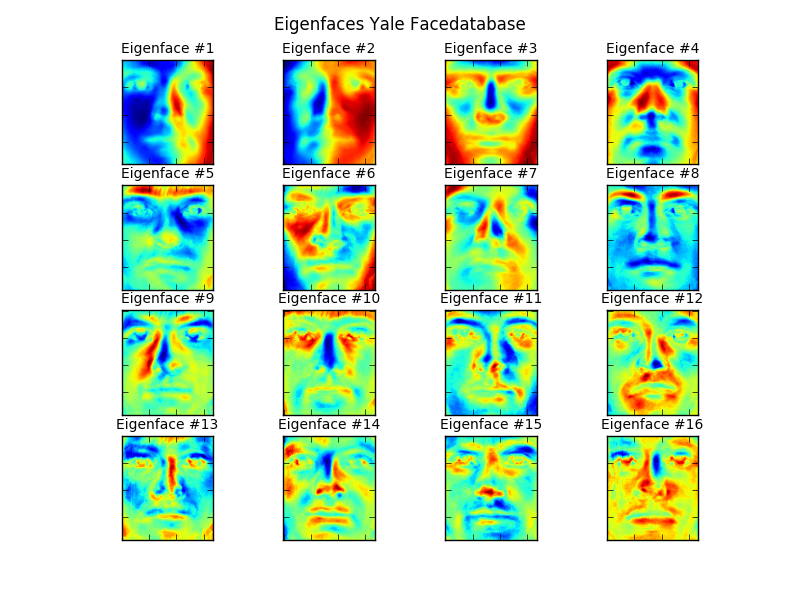
\includegraphics[width=0.8\linewidth]{../image/eigenfacesYale.png}\\
\end{center}

上面这张图抽取了PCA中的前16个特征向量并且还原成人脸,可以看到很多特征向量收到光照的污染非常严重。因此,在PCA中,将受污染的特征向量丢弃,会有助于提高识别率。如何找到这些受污染的特征向量就是另一个话题了。\\

而对于卷积网络,由于它对于人脸特征的抽象层次较高,能够过滤掉一些光照干扰,所以识别率依然接近$100\%$。

\subsection{人脸识别系统}

人脸识别系统是一个非常复杂的工程。如果能在实际中应用,需要结合摄像技术、计算机视觉、机器学习等诸多领域的内容。就以公安系统的人脸识别为例,需要通过摄像头抓取图像,然后能够对图像剪裁,将不同的人脸分辨出来。然后通过与数据库中的储存的犯罪嫌疑人的照片进行学习、识别。每一个过程,考虑到数据量和实际应用场景,都是很复杂的,不同于上面两个模型试验,需要计算机科学家与工程师们的不懈努力。

\section{参考资料}

Stanford, CS231n, Computer Vision\\
github.com/bytefish/facerecognition guide\\
Keras, https://keras.io/
AT\&T数据集\\
Yale数据集\\





\end{document}